\chapter{Introduction}

{\sf What is machine learning? The good answer is <<noone knows>>. However, we know whether or not this particular thing is machine learning or not. Another answer was proposed in the 90's by Arthur Samuel, one of the fathers of machine learning:
\begin{displayquote}
  \glqq It is a field of study that gives the ability to the computer to self-learn without being explicitly programmed.\grqq
  \begin{flushright}
  	A.L. Samuel
  \end{flushright}
\end{displayquote}
}

\section{Types of Machine Learning}

Here we can see some classification of mahine learning situations:
\begingroup
	\def\arraystretch{2}
	\begin{figure}[H]
		\centering
		\begin{tabular}{|c|c|c|} 
			\hline
			{\bf Type} & {\bf Small data} & {\bf Big data} \\
			\hline
			{\bf Panel data} & kNN, SVM, linear regression & boosted decision trees \\
 			\hline
 			{\bf Images, sound, text} & deep learning with tricks & deep learning \\
	 		\hline
	 		{\bf Cluster analysis} &  & clustering methods \\
	 		\hline
	 		{\bf Optimization} & Bayesian optimization & hill climb, annealing, GA\\
	 		\hline
	 		{\bf Agent systems} & q-learning & deep RL \\
 			\hline
		\end{tabular}
	\end{figure}
\endgroup
So the focus of this cource is practical knowledge. There is some theory to machine learning and in most situations theory doesn't work. <<Theory doesn't work>> means <<theory won't tell you what method is the best for particular task>>. Theoreticaly we can say that some method is better than other with probability 51\% but for particular task we may not know what method is the best. So you should know most of the algorithms and apply all of them for your task to find the optimal one.\\
Also there is an another classification of machine learning tasks -- classification by a data structure.

\subsubsection*{Supervised learning}

We have some dataset and we have superviser what tells us <<what is what>>, for example, we have some dataset of handwritten digits and superviser parses this digits. \\
So we have:
\begin{enumerate}[label=$\bullet$]
	\item $x$ -- input point
	\item $y$ -- output (or label)
	\item $f\colon X\to Y$ -- target function what we are trying to predict.
	\item $D=\{(x_1,y_1),\ldots(x_N,y_N)\}$ -- data for training; $x_i$ is the vector (for example, values of the pixel of the image), $y_i$ is the label of element $x_i$.
	\item $h\colon X\to Y$ -- hypothesis, the answer of our algorithm.
\end{enumerate}
Classification problem -- $y$ belongs to a set of classes.\\
Regression problem -- $y$ is a real valued number (or a vector).

\subsubsection*{Unsupervised learning}

Unsupervised learning is when you have only the datapoints $X$ and you want to extract some information, to get some insight into data structure, to get dependences or just for compressing. 

\subsubsection*{Semi-supervised learning}

Let's imagine you have some vector space and you have two data points: black and white. And you want to predict color for other points.

\subsubsection*{Active learning}

It is like semi-supervised learning, but we can ask for more labels but do it on a budget.

\subsubsection*{Reinforcement learning}

You don't have the dataset, you only have an environment and an agent that interacts with this environment and receives some revard. The task is find the best strategy for that environment.

\section{Instance-Based Learning}

In instance-based learning (also lazy learning) class $y$ of point $x$ will be
$$h(x, D)=\arg\max\limits_{y\in Y}\Gamma_y(x), \qquad \Gamma_y(x)=\sum\limits_{x_i\in D}\mathbb{1}(y=y_i)\cdot w(x_i,x)$$
where $D$ is our dataset, $w(x_i,x)$ weight of point $x_i$ for point $x$ (for example, distance between $x$ and $x_i$), $\Gamma_y(x)$ -- affinity of $x$ to class $y$.

\subsubsection*{Classifier evaluation}

Let's define for each class $y$ and our hypothesis $h(x, D)$:
\begin{enumerate}[label=$\bullet$]
	\item TP (true positive) -- number of points $x_i$ from dataset $D$ such as $h(x_i, D)=y_i=y$;
	\item TN (true negative) -- $h(x_i, D)\ne y$, $y_i\ne y$;
	\item FP (false positive) -- $h(x_i, D)=y$, $y_i\ne y$;
	\item FN (false negative) -- $h(x_i, D)\ne y$, $y_i=y$.
\end{enumerate}
Now we can define some metrics:
\begin{enumerate}[label=$\bullet$]
	\item Presicion (positive predicted value): $$\frac{TP}{TP + FP}$$
	\item Recall (true positive rate): $$\frac{TP}{TP+FN}$$
	\item False positive rate: $$\frac{FP}{TN+FP}$$
	\item Accuracy: $$\frac{TP+TN}{TP+FP+TN+FN}$$
	\item $F_1$ score: $$\frac{2}{\frac{1}{\text{Recall}}+\frac{1}{\text{Presicion}}}$$
\end{enumerate}

\subsubsection*{Train/Test}

If we have some hyperparameters of our classifier (for example, the number of neighbors in kNN), we want to find the optimal ones.
\begin{enumerate}
	\item Put aside a part of a dataset ($\approx 10\%-20\%$) for testing (test dataset);
	\item Train classifier on other part (training dataset);
	\item Optimize hyperparameters of classifier looking at the accuracy on the test dataset.
\end{enumerate}
If you have several different classifiers (and you want to find the best one for your task), it is a bad idea to compare them on a test dataset (what you used to find the best hyperparameters), because of overfitting. Put aside one more dataset (validation dataset).

\subsubsection*{Train/Validate/Test}

\begin{enumerate}
	\item Put aside a part of a dataset ($\approx 10\%-20\%$) for validation (validation dataset) and a part for testing (test dataset);
	\item Train classifier on other part (training dataset);
	\item Optimize hyperparameters of classifier looking at the accuracy on the validation dataset.
	\item Compare classifiers on the test dataset.
\end{enumerate}

\subsubsection*{Cross-validation}

If you have a small dataset, you want to use all your dataset for training and all your dataset for testing. And what we do is we shuffle the dataset, separate it into five parts and we make five experiments with same classifier hyperparameters (in k'th experiment we use k'th part for testing and others for training) and the acuracy will be the average of accuracies of each experiment.

\newpage
\subsubsection*{Pareto efficiency}

\begin{wrapfigure}{r}{0.25\linewidth}
	\vspace{-1.25cm}
  \begin{center}
    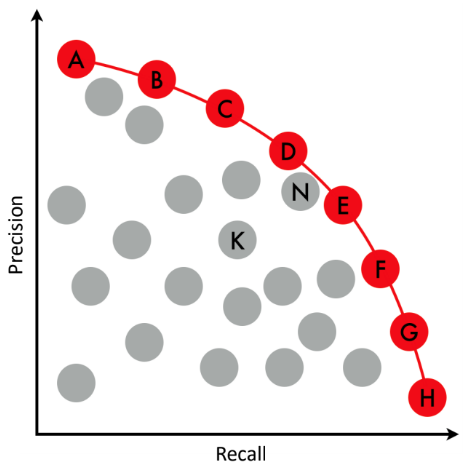
\includegraphics[width=\linewidth]{1a.png}
  \end{center}
  \vspace{-0.8cm}
  \caption*{(1.1) Pareto efficiency}
  \vspace{-1cm}
\end{wrapfigure}
Let's imagine we have some various classifiers and let's look on theirs presicion and recall [pic. 1.1.]. A classifier is Pareto efficient if there is no better classifier in terms of both presicion and recall (red points and point $N$). The red points are the first Pareto frontiers (point $N$ is one of the second Pareto frontiers, $K$ -- third).

\subsubsection*{Scalers}

If one feature goes from 0 to 1000 and the second feature goes from 0 to 1, then when we calculate distances between points, we will use only first feature. To fight that we can use scalers:
\begin{enumerate}[label=$\bullet$]
	\item MinMax scaler: $$x_{scaled}=\frac{x-\min(X)}{\max(X)-\min(X)}$$
	\item MaxAbs scaler: $$x_{scaled}=\frac{x}{\max(|X|)}$$
	\item Standart scaler: $$x_{scaled}=\frac{x-\text{mean}(X)}{\text{std}(X)}$$ where std$(X)$ is the standart deviation.
	\item Robust scaler: $$\frac{x-\text{median}(X)}{\text{percentile}_{0.75}(X)-\text{percentile}_{0.25}(X)}$$
	Robust scaler helps us to avoid points what are far from others.
\end{enumerate}
[Важное уточнение: если мы поделили датасет на две части (для обучения и для тестирования), то мы нормализуем не по всему набору данных, а отдельно для тестовой выборки и отдельно для обучающей.]

\subsubsection*{DROP5}

Prototype selection is calculating $h(x_i, D)$ not over all dataset $D$ but rather its subset $\Omega$. How we should select that subset? There are a lot methods and one of most popular is DROP5 (Decremental Reduction Optimization Procedure):
\begin{figure}[H]
  \centering
  \begin{subfigure}[c]{0.3\linewidth}
    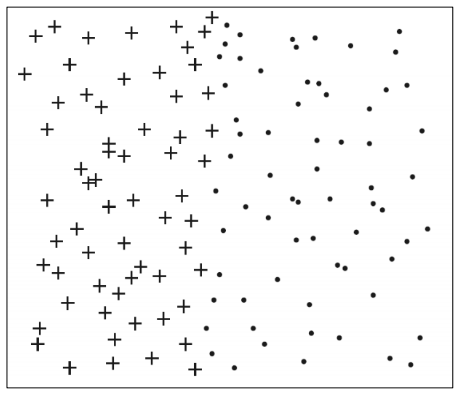
\includegraphics[width=\linewidth]{1b.png}
    \caption*{Dataset}
  \end{subfigure}
  \hspace{2cm}
  \begin{subfigure}[c]{0.3\linewidth}
    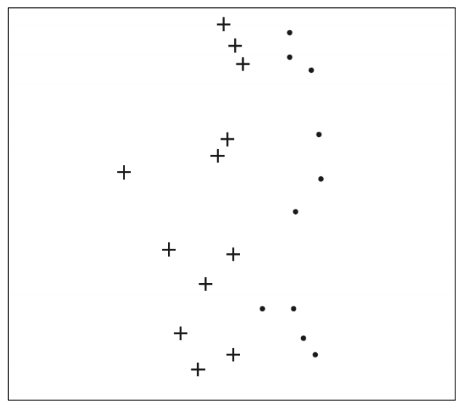
\includegraphics[width=\linewidth]{1c.png}
    \caption*{After DROP5}
  \end{subfigure}
\end{figure}
\begin{enumerate}
	\item Start with the full dataset.
	\item Sort data points, for example, by the number of neighbors from the other class.
	\item Go in the ascending order. Delete point $x$ if that does not increase the LOO error for the points that consider $x$ one of their closest neighbors.
\end{enumerate}

\section{kNN}

In kNN (k-nearest neighbors)
$$h_k(x, D)=\arg\max\limits_{y\in Y}\sum\limits_{x_i\in D}\mathbb{1}(y=y_i)\cdot w_k(x_i,x)$$
$$w_k(x_i,x)=\begin{cases}
	1, & \text{if $x_i$ -- one of the k nearest neighbors of $x$} \\
	0. & \text{otherwise}
\end{cases}
$$
Another variant is radius neighbors:
$$w_k(x_i,x)=\begin{cases}
	1, & \text{if distance $\rho(x_i,x)<R$} \\
	0. & \text{otherwise}
\end{cases}
$$
Actually we don't need a metric space, we only need $\rho(x_i, x)$ (distance between $x_i$ and $x$) to be defined. \\
And the way to evaluate how we are performing is to calculate leave-one-out-error:
$$LOO(k,D)=\frac{1}{|D|}\sum\limits_{x_i\in D}\mathbb{1}(h_k(x_i,D\backslash\{x_i\})\ne y_i)$$

\subsubsection*{WkNN}

Also we can use some other functions $w(x_i,x)=K(\rho(x_i,x)/r)$:
$$K=\max\Big(\frac{r-\rho(x_i,x)}{r}, 0\Big)\qquad K=q^{-\rho(x_i,x)}$$
where $r$ is some constant. We can define $r$ as a distance between $x$ and it's $(k+1)$ nearest neighbor.\\
Also there is a potential energy method:
$$h(x, D)=\arg\max\limits_{y\in Y}\sum\limits_{x_i\in D}\mathbb{1}(y=y_i)\cdot\gamma_i K\left(\frac{\rho(x_i,x)}{r_i}\right)$$
where $\gamma_i$ is some weight of point $x_i$, $r_i$ (influence range of point $x_i$) -- some constant. So we initialize $\gamma_i=0$ and after each step we change $\gamma_i$ ($\gamma_i\to\gamma_i+1$) if $h(x_i, D)\ne y_i$. And after some steps we stop.

\subsubsection*{Step-wise kNN}

If points of our dataset are from a big dimensional space, the euclidian distances between points may be huge. And if we also want to use kNN, the way to do it is the step-wise kNN:
\begin{enumerate}
	\item Select the best feature $k$ (what gives the best kNN result). Now we define the distance $\rho(x_i, x_j)$ between points $x_i$ and $x_j$ as the distance $\rho_k(x_i,x_j)$ between their k'th features.
	\item Find another best feature $k'$ and the weight $w_{k'}$ (what gives the best kNN result). Now we redefine $\rho(x_i,x_j)=\rho(x_i,x_j)+w_{k'}\rho_{k'}(x_i,x_j)$.
	\item Repeat second step while the LOO is decreasing (or the accuracy is increasing).
\end{enumerate}